
\documentclass{beamer}
\usepackage{beamerthemeshadow}
\usepackage[english]{babel}

\begin{document}
\title{Modeling Variable Throughput Channels with Stochastic ODEs}  
\author{D. Masi, P. Pegus II , J. Wong}
\date{\today} 

\frame{\titlepage} 

\frame{\frametitle{Outline}\tableofcontents} 

\section{Introduction} {
	\frame{\frametitle{Introduction} {
		\begin{figure}[H]
		\centering
		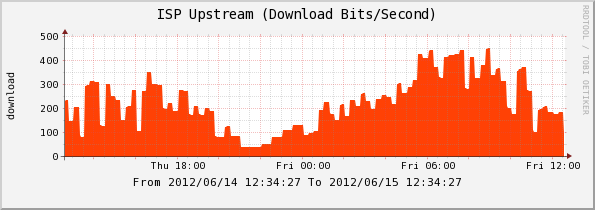
\includegraphics[scale=.40]{Images/throughput.png}
		\end{figure}
		Stochastic differential equations are often used to model the nondeterministic behavior of network channels in computer science.
		}
	}
}
\section{Networking Basics} {
	\frame{\frametitle{Networking Basics} {
		A \textbf{Channel} is the medium through which a message propagates from sender to receiver.
		\begin{figure}[H]
		\centering
		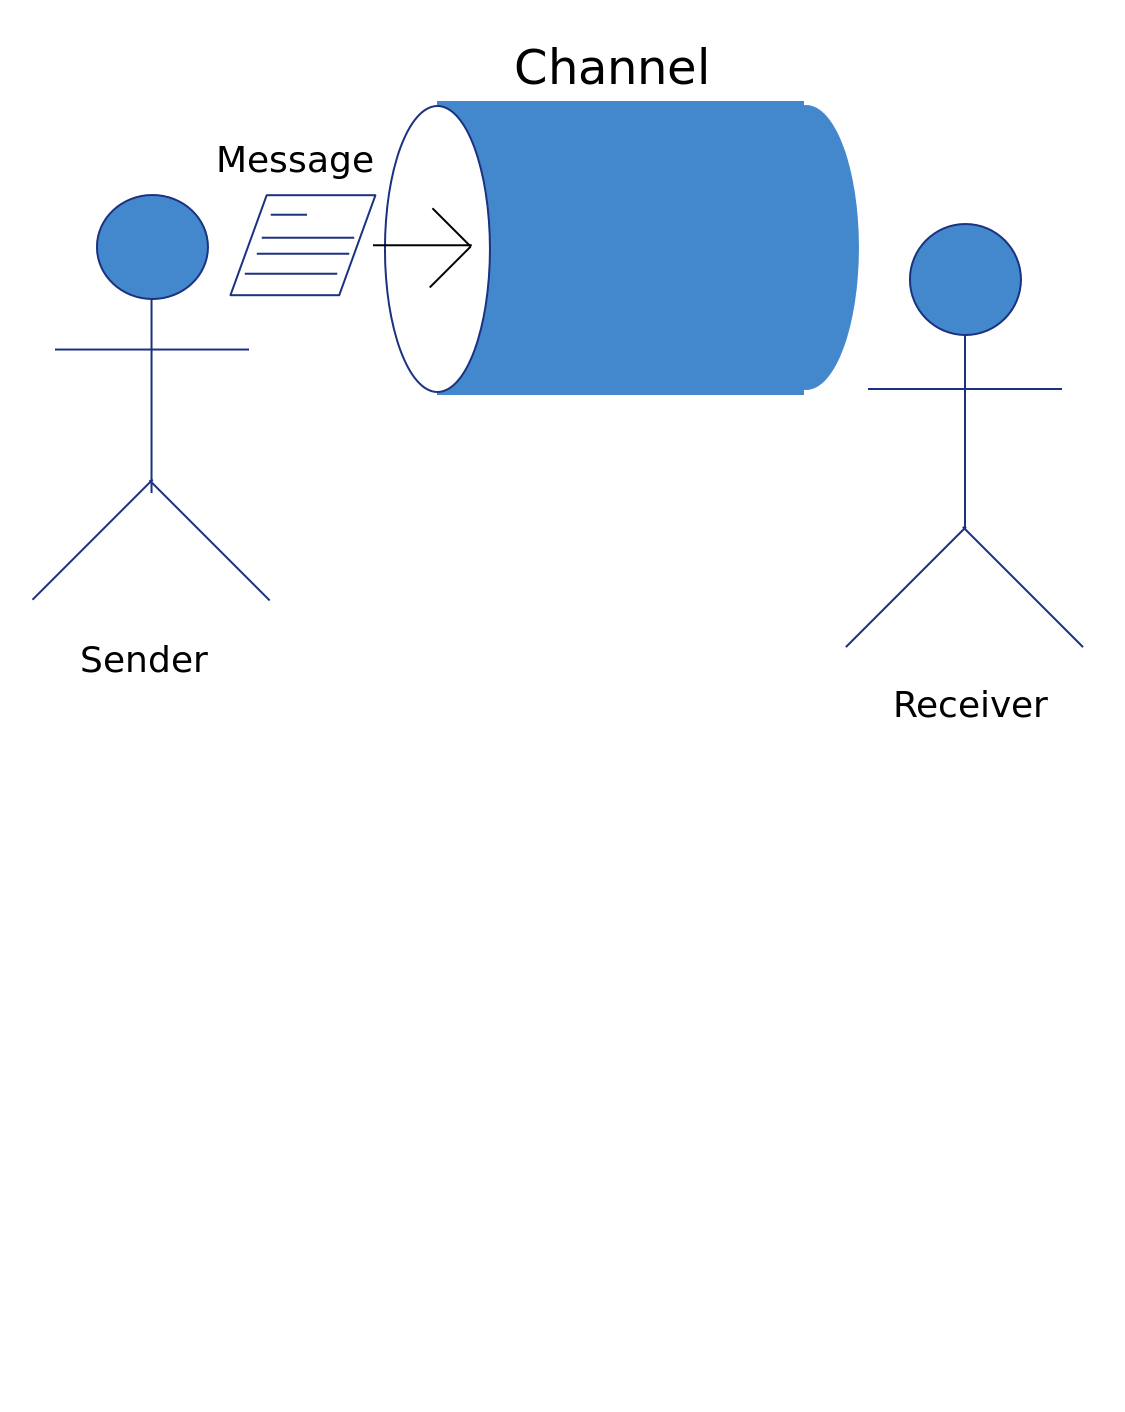
\includegraphics[scale=.20]{Images/network_components.png}
		\end{figure}
		}
	}
}
\section{Channel Characteristics} {
	\frame{\frametitle{Channel Characteristics} {
		\begin{figure}[H]
		\centering
		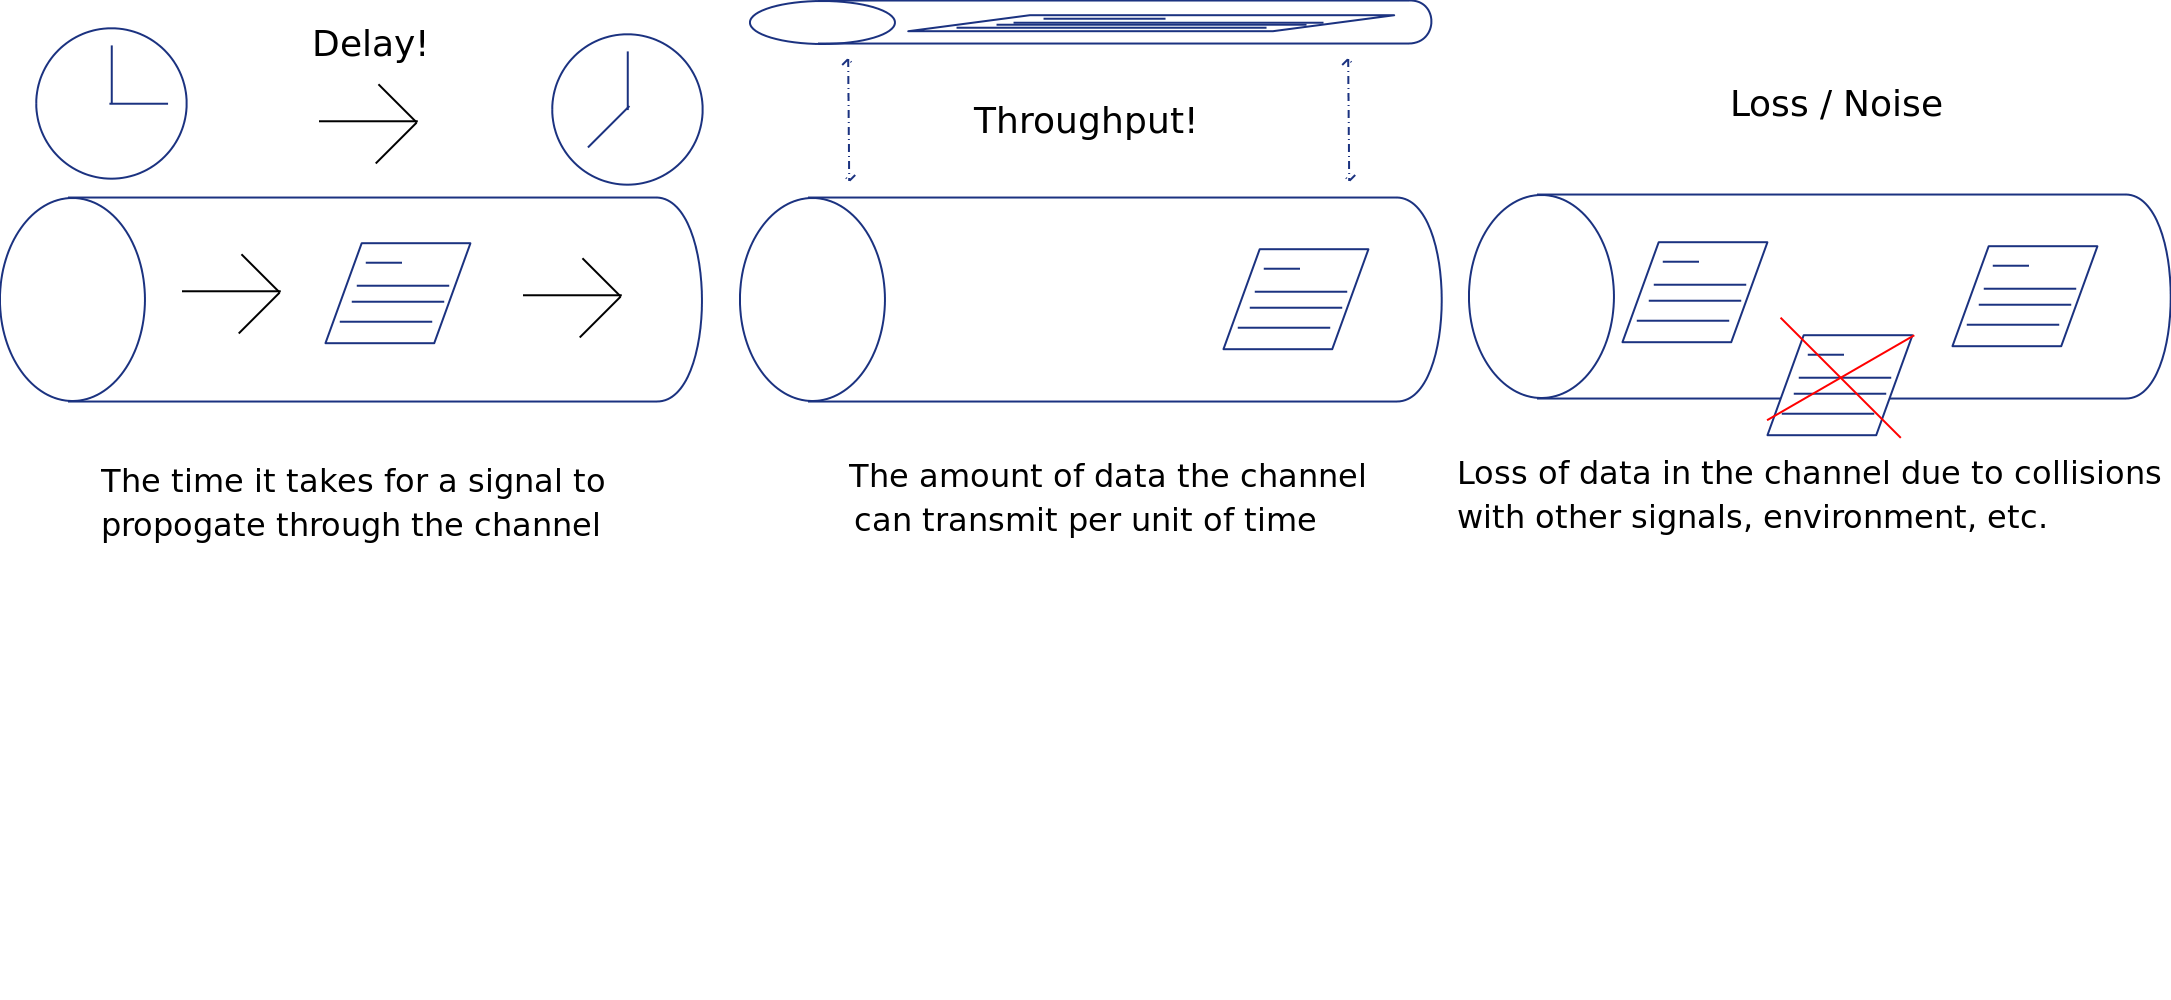
\includegraphics[scale=.15]{Images/channel_characteristics.png}
		\end{figure}
		}
	}
}
\section{Demonstration}{
	\frame{\frametitle{Demonstration} {
		\begin{figure}[H]
		\centering
		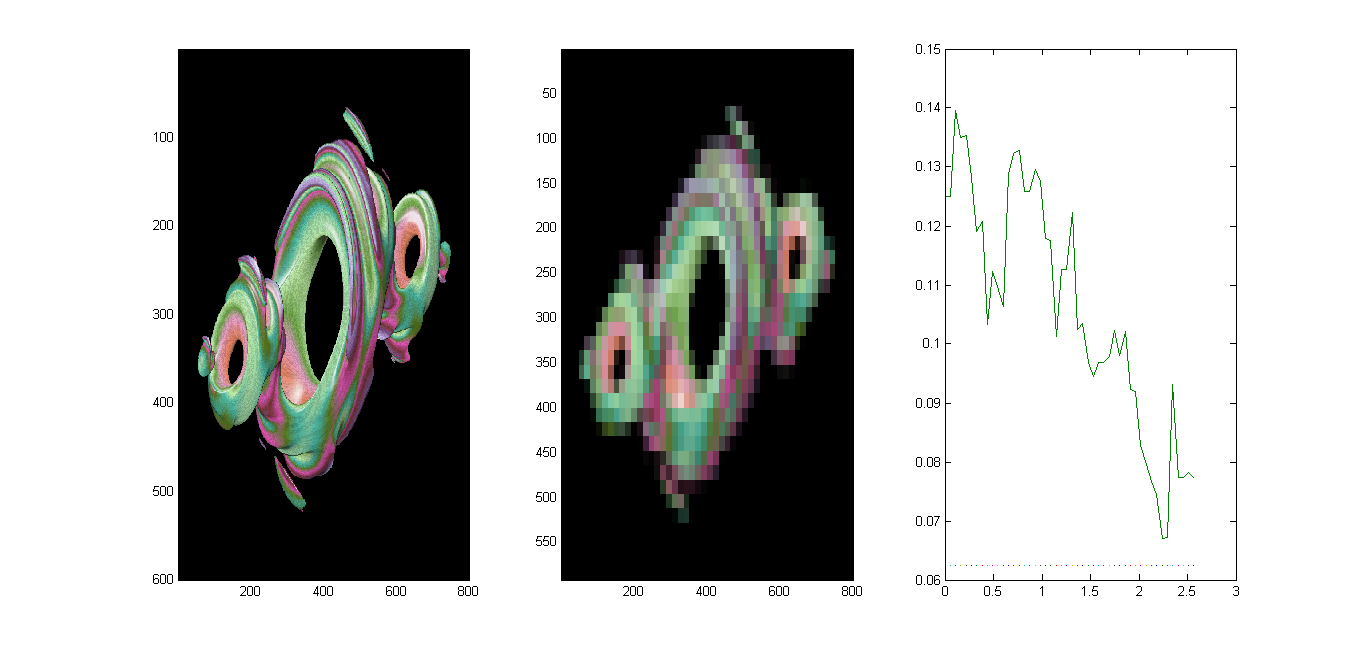
\includegraphics[scale=.30]{Images/img.png}
		\end{figure}
}

}

}

\end{document}
\section{Demonstration}{
	\frame{\frametitle{Demonstration} {
		\begin{figure}[H]
		\centering
		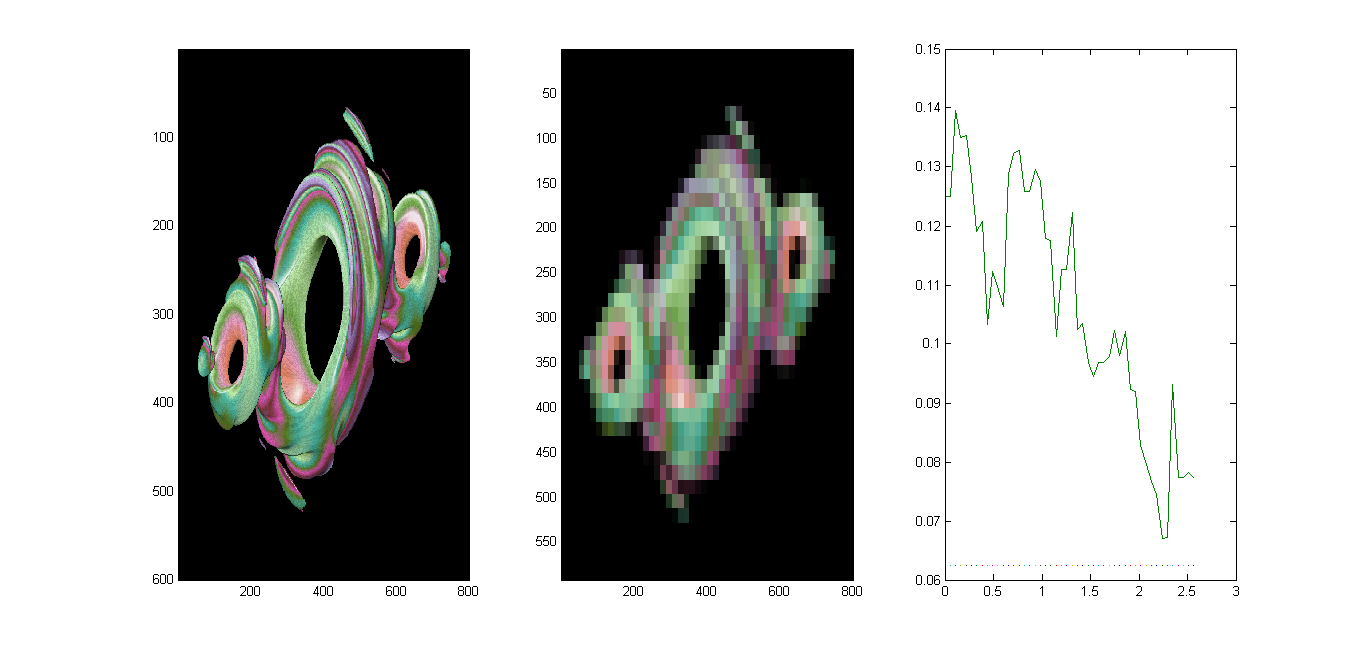
\includegraphics[scale=.30]{Images/img.png}
		\end{figure}
}

}

}

\end{document}

